\clearpage
\appendix
\section{Technical Appendix}
\strex*
\begin{proof}
   That the strategy existence problem is in NP follows from the fact that model checking $\mathcal{L}^n$ is in P. Indeed, since the mechanism is finite and sellers have a finite budget, there is an upper bound on the length of $\langle \overline{\sigma}: \overline{\beta} \rangle^\ast$. In particular, the length of $\langle \overline{\sigma}: \overline{\beta} \rangle^\ast$ is polynomial in the size of $M$ (in the worst case, each seller incentivises each buyer and the total number of incentivisations is bounded by sellers' budgets that are a part of the input). Therefore, we can guess a sequence $\langle \overline{\sigma}: \overline{\beta} \rangle^\ast$ of at most polynomial size, and then verify $M,s \models \langle \overline{\sigma}: \overline{\beta} \rangle^\ast \varphi$ for sellers $s \in S$ in polynomial time.

    For NP-hardness, it is enough to show only the case of the single seller mechanism. To this end, we employ a reduction from 3-SAT. Let $\Psi = \bigwedge_{1 \leqslant i \leqslant k} \beta_i$ be a 3-SAT instance with $\beta_i = \gamma^i_1 \lor \gamma^i_2 \lor \gamma^i_3$, where $\gamma^i$ are literals. Moreover, let $\Delta = \{\delta_1,..., \delta_n\}$ be the set of atoms occurring in $\Psi$.

    Given a $\Psi$, we will construct a 1-DAM $M_\Psi$ with arbitrary polynomially computable $P$, $\Pay$, $Ut$. The set of agents $Agt = \{s, b_1,...,b_k,$ $c^1_{1,1}, c^1_{2,1}, c^1_{3, 1}, ....,$ $c^k_{3, n}, d_1,...,$ $d_n, e^1_1, e^1_2, ..., e^n_1, e^n_2, t_1, ..., t_n, f_1, ..., f_n\}$, where $s$ is the seller, agents $b_i$ correspond to clauses in $\Psi$, agents $c^i_{j,l}$ correspond to literals in a given clause $i$ with $j$ being the position of the literal in the clause and $l$ the number of the corresponding atom from $\Delta$, agents $d_i$ correspond to atoms in $\Delta$, agents $e^i_j$ help to split the valuations of atoms, and $t_i$ and $f_i$ correspond to setting the corresponding atom to \textit{true} or \textit{false}. Relation $F$ is set up in a hierarchical way, with $F(s, \{b_i | 1 \leqslant i \leqslant k\})$, $F(b_i, \{c^i_{1,l}, c^i_{2,l'}, c^i_{3,l''}\})$ for all $b_i$, $F(c^i_{j,l}, d_l)$ for all $c^i_{j,l}$ such that $d_l$ is the corresponding atom for literal $c^i_{j,l}$, $F(d_i, \{e^i_1, e^i_2\})$ for all $d_i$, and $F(e^i_1, t_i)$ and $F(e^i_2, f_i)$ for all $e^i_j$. Further, $Bdg$ and $V$ are defined arbitrarily, and $I(a) = 0$ for all $a\in Agt$. Finally, $N(\sigma) = s$, $N(\beta_i) = b_i$, $N(\gamma^i_{j,l}) = c^i_{j,l}$ if the corresponding literal is positive and $N(\overline{\gamma^i_j}) = c^i_j$ otherwise, $N(\delta_i) = d_i$, $N(\epsilon^i_j) = e^i_j$,  $N(true_i) = t_i$, and $N(false_i) = f_i$. All other names are distributed arbitrarily\footnote{The reader might have noticed that we use the same symbols for atoms in $\Psi$ and names of $d$-agents. This is done on purpose to make Figure \ref{fig:satexample} more readable and to highlight that $d$-agents correspond to atoms. Similarly for clauses and literals.}.

    As an example of the construction, consider the 3-SAT instance $\Psi = (\delta_1 \lor \delta_2 \lor \delta_3) \land (\lnot \delta_1 \lor \delta_3 \lor \lnot \delta_4)$, and the corresponding mechanism $M_\Psi$ in Figure \ref{fig:satexample}.  

    \begin{figure}[h!]
\centering
\scalebox{0.8}{
   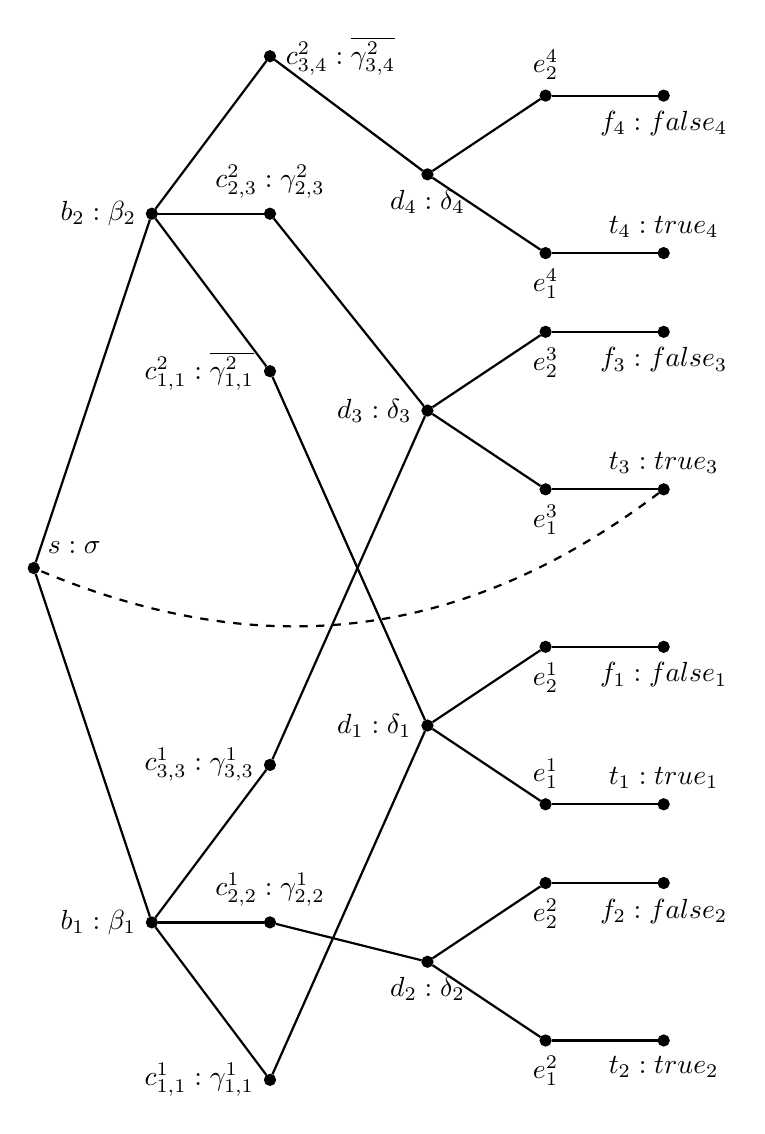
\begin{tikzpicture}[rotate = 90]
\node[circle,draw=black, minimum size=4pt,inner sep=0pt, fill = black, label=above right:{$s:\sigma$}](s) at (0,0) {};
\node[circle,draw=black, minimum size=4pt,inner sep=0pt,, fill = black , label=left:{$b_1:\beta_1$}](b1) at (-4.5,-1.5) {};
\node[circle,draw=black, minimum size=4pt,inner sep=0pt, , fill = black, label=left:{$b_2:\beta_2$}](b2) at (4.5,-1.5) {};
\node[circle,draw=black, minimum size=4pt,inner sep=0pt,, fill = black , label=left:{$c_{1,1}^1:\gamma_{1,1}^1$}](c11) at (-6.5,-3) {};
\node[circle,draw=black, minimum size=4pt,inner sep=0pt,, fill = black , label=above:{$c_{2,2}^1:\gamma_{2,2}^1$}](c12) at (-4.5,-3) {};
\node[circle,draw=black, minimum size=4pt,inner sep=0pt,, fill = black , label=left:{$c_{3,3}^1:\gamma_{3,3}^1$}](c13) at (-2.5,-3) {};

\node[circle,draw=black, minimum size=4pt,inner sep=0pt,, fill = black , label=right:{$c_{3,4}^2:\overline{\gamma_{3,4}^2}$}](c23) at (6.5,-3) {};
\node[circle,draw=black, minimum size=4pt,inner sep=0pt,, fill = black , label=above:{$c_{2,3}^2:\gamma_{2,3}^2$}](c22) at (4.5,-3) {};
\node[circle,draw=black, minimum size=4pt,inner sep=0pt,, fill = black , label=left:{$c_{1,1}^2:\overline{\gamma_{1,1}^2}$}](c21) at (2.5,-3) {};

\node[circle,draw=black, minimum size=4pt,inner sep=0pt,, fill = black , label=below:{$d_2:\delta_2$}](d2) at (-5,-5) {};
\node[circle,draw=black, minimum size=4pt,inner sep=0pt,, fill = black , label=left:{$d_1:\delta_1$}](d1) at (-2,-5) {};
\node[circle,draw=black, minimum size=4pt,inner sep=0pt,, fill = black , label=left:{$d_3:\delta_3$}](d3) at (2,-5) {};
\node[circle,draw=black, minimum size=4pt,inner sep=0pt,, fill = black , label=below:{$d_4:\delta_4$}](d4) at (5,-5) {};

\node[circle,draw=black, minimum size=4pt,inner sep=0pt,, fill = black , label=below:{$e^2_1$}](e21) at (-6,-6.5) {};
\node[circle,draw=black, minimum size=4pt,inner sep=0pt,, fill = black , label=below:{$e^2_2$}](e22) at (-4,-6.5) {};
\node[circle,draw=black, minimum size=4pt,inner sep=0pt,, fill = black , label=above:{$e^1_1$}](e11) at (-3,-6.5) {};
\node[circle,draw=black, minimum size=4pt,inner sep=0pt,, fill = black , label=below:{$e^1_2$}](e12) at (-1,-6.5) {};
\node[circle,draw=black, minimum size=4pt,inner sep=0pt,, fill = black , label=below:{$e^3_1$}](e31) at (1,-6.5) {};
\node[circle,draw=black, minimum size=4pt,inner sep=0pt,, fill = black , label=below:{$e^3_2$}](e32) at (3,-6.5) {};
\node[circle,draw=black, minimum size=4pt,inner sep=0pt,, fill = black , label=below:{$e^4_1$}](e41) at (4,-6.5) {};
\node[circle,draw=black, minimum size=4pt,inner sep=0pt,, fill = black , label=above:{$e^4_2$}](e42) at (6,-6.5) {};

\node[circle,draw=black, minimum size=4pt,inner sep=0pt,, fill = black , label=below:{$t_2:true_2$}](t2) at (-6,-8) {};
\node[circle,draw=black, minimum size=4pt,inner sep=0pt,, fill = black , label=below:{$f_2:false_2$}](f2) at (-4,-8) {};
\node[circle,draw=black, minimum size=4pt,inner sep=0pt,, fill = black , label=above:{$t_1:true_1$}](t1) at (-3,-8) {};
\node[circle,draw=black, minimum size=4pt,inner sep=0pt,, fill = black , label=below:{$f_1:false_1$}](f1) at (-1,-8) {};
\node[circle,draw=black, minimum size=4pt,inner sep=0pt,, fill = black , label=above:{$t_3:true_3$}](t3) at (1,-8) {};
\node[circle,draw=black, minimum size=4pt,inner sep=0pt,, fill = black , label=below:{$f_3:false_3$}](f3) at (3,-8) {};
\node[circle,draw=black, minimum size=4pt,inner sep=0pt,, fill = black , label=above:{$t_4:true_4$}](t4) at (4,-8) {};
\node[circle,draw=black, minimum size=4pt,inner sep=0pt,, fill = black , label=below:{$f_4:false_4$}](f4) at (6,-8) {};


\draw[thick] (s) to (b1);
\draw[thick] (s) to (b2);

\draw[thick] (c11) to (b1);
\draw[thick] (c12) to (b1);
\draw[thick] (c13) to (b1);

\draw[thick] (c21) to (b2);
\draw[thick] (c22) to (b2);
\draw[thick] (c23) to (b2);

\draw[thick] (c11) to (d1);
\draw[thick] (c21) to (d1);
\draw[thick] (c12) to (d2);
\draw[thick] (c13) to (d3);
\draw[thick] (c22) to (d3);
\draw[thick] (c23) to (d4);

\draw[thick] (e11) to (d1);
\draw[thick] (e12) to (d1);
\draw[thick] (e21) to (d2);
\draw[thick] (e22) to (d2);
\draw[thick] (e31) to (d3);
\draw[thick] (e32) to (d3);
\draw[thick] (e41) to (d4);
\draw[thick] (e42) to (d4);

\draw[thick] (e11) to (t1);
\draw[thick] (e12) to (f1);
\draw[thick] (e21) to (t2);
\draw[thick] (e22) to (f2);
\draw[thick] (e31) to (t3);
\draw[thick] (e32) to (f3);
\draw[thick] (e41) to (t4);
\draw[thick] (e42) to (f4);

\draw[thick,dashed, bend left] (t3) to (s);


\end{tikzpicture}
 }
\caption{Mechanism $M$ for the 3-SAT instance $\Psi$ with one new link being dashed, and other new links being omitted for readability.}
\label{fig:satexample}
\end{figure} 

As for goal formula $\varphi_\Psi$, we take $$\varphi_\Psi = \square %\bigwedge_{1\leqslant i \leqslant k}
\left( \beta_i \to \Diamond %\bigvee_{j \in \{1,2,3\}} 
\left((\gamma^i_{j,l} \lor \overline{\gamma^i_{j,l}}) \land \psi_0 \land \psi_1\right)\right)$$
$\text{ for } 1\leqslant i \leqslant k, 1 \leqslant j \leqslant 3 \text { and } 1 \leqslant l \leqslant n$,
where $$\psi_0 = \overline{\gamma^i_{j,l}} \to (\Diamond \Diamond \Diamond (%\bigvee_{1\leqslant l \leqslant n} 
false_l \land \Diamond \sigma) \land \lnot \Diamond \Diamond \Diamond (%\bigvee_{1\leqslant l \leqslant n} 
true_l \land \Diamond \sigma))$$ $$\psi_1 = \gamma^i_{j,l} \to (\Diamond \Diamond \Diamond (%\bigvee_{1\leqslant l \leqslant n} 
true_l \land \Diamond \sigma) \land  \lnot \Diamond \Diamond \Diamond (%\bigvee_{1\leqslant l \leqslant n} 
false_l \land \Diamond \sigma)).$$

The goal formula is constructed in such a way in order to mimic, together with the model $M_\Psi$, the instance of 3-SAT $\Psi$. Hence, it is easy to verify that there is a sequence of incentives for the seller such that $M_\Psi, s \models \langle \alpha \rangle^\ast \varphi_\Psi$ if and only if $\Psi$ is satisfiable. Indeed, to satisfy $\Psi$ we need to satisfy all its clauses, which, in the goal formula, corresponds to the fact that we visit all friends of $s$ with names $\beta_i$. Then, for each clause, we need to find at least one literal, positive or negative, which is true. In the goal formula, this corresponds to checking the existence of a at least one friend (of three total) of a given $\beta_i$ which is a literal (part $\gamma^i_{j,l} \lor \overline{\gamma^i_{j,l}}$), and if the literal is negative (case $\psi_0$), then the corresponding \textit{false} agent is reachable that participates in the auction, and no corresponding \textit{true} agent is reachable such that the agent is friends with the seller (i.e. that the truth value of the corresponding atom is set only to \textit{false}). Similarly for $\psi_1$. 

In other words, if $\Psi$ is satisfiable, then an atom $\delta_i$ in $\Psi$ is true if and only if the corresponding $t_i$ agent participates in the auction. And vice versa, if there is a sequence of incentives that satisfies the goal formula, then we set an atom $\delta_i$ in $\Psi$ to true if and only if the corresponding $t_i$ agent is participating in the auction.  

For the given example of $\Psi$, the sellers strategy could be $\langle \beta_1\rangle \langle \gamma^1_{3,3} \rangle \langle \delta_3 \rangle \langle \epsilon_1^3 \rangle$, and the result of executing such a strategy is presented in Figure \ref{fig:satexample} (with one dashed new line, all other new lines are omitted for readability). It is easy to verify that in the updated mechanism, the goal formula holds, which, for the given example, corresponds to setting atom $\delta_3$ to true and thus satisfying $\Psi$.
\end{proof}

\slexp*
\begin{proof}
         %That $\mathcal{SL}^n$ is at least as expressive as $\mathcal{L}^n$ follows from the fact that $\mathcal{L}^n \subset \mathcal{SL}^n$. Now we 
         We need to show that there is a formula of $\mathcal{SL}^n$ for which there is no equiavalent formula of $\mathcal{L}^n$. Consider $\langle \! [ \sigma ] \! \rangle \Diamond \gamma \in \mathcal{SL}^1$ constructed over the single seller, and assume towards a contradiction that there is an equivalent formula $\varphi \in \mathcal{L}^1$. Recall that $name(\varphi)$ be the set of nominals appearing in $\varphi$. The set is finite since $\varphi$ is finite. 
     
     Now consider the following two 1-DAMs depicted in Figure \ref{fig:exprproof}, where $\alpha_1,...,\alpha_n$ are all buyer names from $name(\varphi) \setminus \{\gamma\}$.
     \begin{figure}[h!]
\centering
\scalebox{0.8}{
   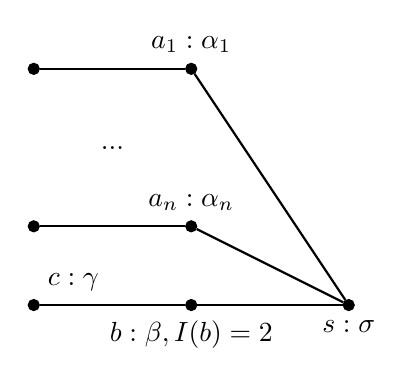
\begin{tikzpicture}[rotate = -90]
\node[circle,draw=black, minimum size=4pt,inner sep=0pt, fill = black, label=below:{$s:\sigma$}](s) at (0,0) {};
\node[circle,draw=black, minimum size=4pt,inner sep=0pt,, fill = black , label=above:{$a_1:\alpha_1$}](a10) at (-3,-2) {};
%\node[circle,draw=black, minimum size=4pt,inner sep=0pt,, fill = black , label=left:{$a_2:\alpha_2$}](a11) at (-1,-2) {};
\node[circle,draw=black, minimum size=4pt,inner sep=0pt, , fill = black, label=below:{$b:\beta, I(b) = 2$}](a21) at (0,-2) {};
\node[circle,draw=black, minimum size=4pt,inner sep=0pt, , fill = black, label=above:{$a_n:\alpha_n$}](a20) at (-1,-2) {};

\node[circle,draw=black, minimum size=4pt,inner sep=0pt,, fill = black ](b10) at (-3,-4) {};
%\node[circle,draw=black, minimum size=4pt,inner sep=0pt,, fill = black ](b11) at (-1,-4) {};
\node[circle,draw=black, minimum size=4pt,inner sep=0pt, , fill = black, label=above right:{$c:\gamma$}](b21) at (0,-4) {};
\node[circle,draw=black, minimum size=4pt,inner sep=0pt, , fill = black](b20) at (-1,-4) {};

\node (dots) at (-2,-3) {$...$};

\draw[thick] (s) to (a10);
%\draw[thick] (s) to (a11);
\draw[thick] (s) to (a20);
\draw[thick] (s) to (a21);

\draw[thick] (b10) to (a10);
%\draw[thick] (b11) to (a11);
\draw[thick] (b20) to (a20);
\draw[thick] (b21) to (a21);

\end{tikzpicture}
\hspace{7mm}
   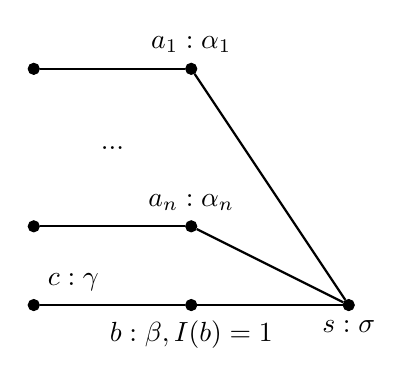
\begin{tikzpicture}[rotate = -90]
\node[circle,draw=black, minimum size=4pt,inner sep=0pt, fill = black, label=below:{$s:\sigma$}](s) at (0,0) {};
\node[circle,draw=black, minimum size=4pt,inner sep=0pt,, fill = black , label=above:{$a_1:\alpha_1$}](a10) at (-3,-2) {};
%\node[circle,draw=black, minimum size=4pt,inner sep=0pt,, fill = black , label=left:{$a_2:\alpha_2$}](a11) at (-1,-2) {};
\node[circle,draw=black, minimum size=4pt,inner sep=0pt, , fill = black, label=below:{$b:\beta, I(b) = 1$}](a21) at (0,-2) {};
\node[circle,draw=black, minimum size=4pt,inner sep=0pt, , fill = black, label=above:{$a_n:\alpha_n$}](a20) at (-1,-2) {};

\node[circle,draw=black, minimum size=4pt,inner sep=0pt,, fill = black ](b10) at (-3,-4) {};
%\node[circle,draw=black, minimum size=4pt,inner sep=0pt,, fill = black ](b11) at (-1,-4) {};
\node[circle,draw=black, minimum size=4pt,inner sep=0pt, , fill = black, label=above right:{$c:\gamma$}](b21) at (0,-4) {};
\node[circle,draw=black, minimum size=4pt,inner sep=0pt, , fill = black](b20) at (-1,-4) {};

\node (dots) at (-2,-3) {$...$};

\draw[thick] (s) to (a10);
%\draw[thick] (s) to (a11);
\draw[thick] (s) to (a20);
\draw[thick] (s) to (a21);

\draw[thick] (b10) to (a10);
%\draw[thick] (b11) to (a11);
\draw[thick] (b20) to (a20);
\draw[thick] (b21) to (a21);

\end{tikzpicture}

 }

\caption{Mechanisms $M_1$ (left) and $M_2$ (right).}
\label{fig:exprproof}
\end{figure} 

In the models, the seller has budget 1 and the incentives required by each her neighbour $a_i$ is 1, i.e. the seller can incentivise only one buyer. Budgets of all buyers are 0. Buyer $b$, whose name $\beta$ does not appear in $names (\varphi)$ (we can assume the existence of such a name as the set of nominals is countably infinite) has incentive 2 in $M_1$ and 1 in the model $M_2$. It is easy to see that $M_1,s \not \models \langle \! [ \sigma ] \! \rangle \Diamond \gamma$, as the only way for the seller to reach buyer $\gamma$ is by incentivising $\beta$ to invite them. Since the seller's budget is 1, they do not have enough resources to do so. At the same time, $M_2,s  \models \langle \! [ \sigma ] \! \rangle \Diamond \gamma$. Again, even though $\beta$ does not appear explicitly in neither $\varphi$ nor in $\langle \! [ \sigma ] \! \rangle \Diamond \gamma$, modality $\langle \! [ \sigma ] \! \rangle$ still quantifies over this name.

To see that $M_1,s\models \varphi$ if and only if $M_2,s \models \varphi$, it is enough to notice that the distributions of names in mechanisms are identical, and, moreover, since $\beta$ does not appear in $\varphi$, $\beta$ is not a part of the dynamic operators. Finally, we cannot spot the difference in the incentives for agent $b$ in the two mechanism without using incentivisations, which is ruled out due to $\beta$ not being a part of $\varphi$. 
\end{proof}

\mcsl*
\begin{proof}
      For PSPACE-hardness, we employ the reduction from the quantified Boolean formula (QBF) problem, which is known to be PSPACE-complete. The problem consists in determining whether a given QBF $\Psi = Q_1 p_1 ... Q_n p_n \psi(p_1,...,p_n)$ with $Q_i \in \{\forall, \exists\}$ is true. Without loss of generality, we assume that there are no free variables in $\Psi$. For the reduction, we will construct a mechanism $M_\Psi$ over one seller and a formula $\varphi_\Psi$ such that QBF $\Psi$ is true if and only if $M_\Psi, s \models \varphi_\Psi$. 

    Given a QBF $\Psi = Q_1 p_1 ... Q_n p_n \psi(p_1,...,p_n)$, mechanism $M_\Psi$ is the tuple with $Agt = \{s, a_1^0,a_1^1, ..., a_n^0, a_n^1, b_1^0, b_1^1, ..., b_n^0, b_n^1\}$ with $s$ being the seller. Relation $F$ is such that $F(s, a_i^j)$ for all $a_i^j$ and $F(a_i^j,b_i^j)$ for all $a_i^j$ and $b_i^j$. $Bdg$ and $V$ are defined arbitrarily, and $I(a,s) = 0$ for all $a \in Agt$. Functions $N(\sigma) = s$, $N(\alpha_i^j) = a^j_i$,  and $N(\beta_i^j) = b^j_i$. All other names are distributed arbitrarily. Finally, the placement, payment, and utility functions are arbitrary. 
    
    Intuitively, mechanism $M_\Psi$ consists of $2n+1$ agents, where agents $a^0_i$ and $b^0_i$ model the setting atom $p_i$ to \textit{false}, and agents $a^1_i$ and $b^1_i$ model the setting atom $p_i$ to \textit{true}. Which truth value of atom $p_i$ is chosen, \textit{true} or \textit{false}, will be determined whether the corresponding buyer is participating in the auction run by the seller $s$.

    We use the following translation of QBF $\Psi$ into a formula of our logic. First, formula $fixed_k$ intuitively means that truth values of first $k$ atoms in $\Psi$ were chosen:
    $$fixed_k = \bigwedge_{1 \leqslant i \leqslant k} (\Diamond \beta_i^0 \leftrightarrow \lnot \Diamond \beta_i^1) \land \bigwedge_{k < i \leqslant n} (\lnot \Diamond \beta^0_i \land \lnot \Diamond \beta^1_i).$$

    Now,
    \begin{align*}
    \varphi_0 &:= \psi(\Diamond \beta^1_1, ..., \Diamond \beta^1_n)\\
\varphi_k &:= 
\begin{cases} 
	[\! \langle \sigma \rangle \!] (fixed_k \to \varphi_{k-1}) &\text{if } Q_k = \forall\\
	\langle \! [ \sigma ] \! \rangle (fixed_k \land \varphi_{k-1}) &\text{if } Q_k = \exists\\
\end{cases}\\
\varphi_\Psi &:= \varphi_{n}.
\end{align*}

What is left to show is that $\Psi = Q_1 p_1 ... Q_n p_n \psi(p_1,...,p_n)$ is satisfiable if and only if $M_\Psi, s \models \varphi_\Psi$. For this, observe that $M_\Psi, s \models \Diamond \beta_i^1$, i.e. the buyer called $\beta^1_i$ is participating in the auction, holds if the the corresponding atom $p_i$ was set to \textit{true}. And similarly for $\beta_i^0$ and setting $p_i$ to \textit{false}. Since there is only a single seller $\sigma$, setting truth values of $p_i$'s happens sequentially one after another. Moreover, again since we have only the single seller, modalities $[\! \langle \sigma \rangle \!]$ (resp. $\langle \! [ \sigma ] \! \rangle$) correspond to universally (resp. existentially) quantifying over $p_i$. Guards $fixed_k$ guarantee that only truth values of only first $k$ atoms were chosen (conjunct $\bigwedge_{k < i \leqslant n} (\lnot \Diamond \beta^0_i \land \lnot \Diamond \beta^1_i)$), and, additionally, that those truth values were chosen unambiguously, i.e. exactly one truth value per atom (conjunct $\bigwedge_{1 \leqslant i \leqslant k} (\Diamond \beta_i^0 \leftrightarrow \lnot \Diamond \beta_i^1)$). Hence, together with $[\! \langle \sigma \rangle \!]$ and $\langle \! [ \sigma ] \! \rangle$, guards $fixed_k$ emulate quantifiers $\forall$ and $\exists$ in a QBF. Finally, the evaluation of the propositional part of the QBF is captured by the participation of the corresponding buyers in the auction. 
\end{proof}


%\clearpage \input{ReproducibilityChecklist}
\clearpage